% GNUPLOT: LaTeX picture with Postscript
\begingroup
  \makeatletter
  \providecommand\color[2][]{%
    \GenericError{(gnuplot) \space\space\space\@spaces}{%
      Package color not loaded in conjunction with
      terminal option `colourtext'%
    }{See the gnuplot documentation for explanation.%
    }{Either use 'blacktext' in gnuplot or load the package
      color.sty in LaTeX.}%
    \renewcommand\color[2][]{}%
  }%
  \providecommand\includegraphics[2][]{%
    \GenericError{(gnuplot) \space\space\space\@spaces}{%
      Package graphicx or graphics not loaded%
    }{See the gnuplot documentation for explanation.%
    }{The gnuplot epslatex terminal needs graphicx.sty or graphics.sty.}%
    \renewcommand\includegraphics[2][]{}%
  }%
  \providecommand\rotatebox[2]{#2}%
  \@ifundefined{ifGPcolor}{%
    \newif\ifGPcolor
    \GPcolortrue
  }{}%
  \@ifundefined{ifGPblacktext}{%
    \newif\ifGPblacktext
    \GPblacktexttrue
  }{}%
  % define a \g@addto@macro without @ in the name:
  \let\gplgaddtomacro\g@addto@macro
  % define empty templates for all commands taking text:
  \gdef\gplbacktext{}%
  \gdef\gplfronttext{}%
  \makeatother
  \ifGPblacktext
    % no textcolor at all
    \def\colorrgb#1{}%
    \def\colorgray#1{}%
  \else
    % gray or color?
    \ifGPcolor
      \def\colorrgb#1{\color[rgb]{#1}}%
      \def\colorgray#1{\color[gray]{#1}}%
      \expandafter\def\csname LTw\endcsname{\color{white}}%
      \expandafter\def\csname LTb\endcsname{\color{black}}%
      \expandafter\def\csname LTa\endcsname{\color{black}}%
      \expandafter\def\csname LT0\endcsname{\color[rgb]{1,0,0}}%
      \expandafter\def\csname LT1\endcsname{\color[rgb]{0,1,0}}%
      \expandafter\def\csname LT2\endcsname{\color[rgb]{0,0,1}}%
      \expandafter\def\csname LT3\endcsname{\color[rgb]{1,0,1}}%
      \expandafter\def\csname LT4\endcsname{\color[rgb]{0,1,1}}%
      \expandafter\def\csname LT5\endcsname{\color[rgb]{1,1,0}}%
      \expandafter\def\csname LT6\endcsname{\color[rgb]{0,0,0}}%
      \expandafter\def\csname LT7\endcsname{\color[rgb]{1,0.3,0}}%
      \expandafter\def\csname LT8\endcsname{\color[rgb]{0.5,0.5,0.5}}%
    \else
      % gray
      \def\colorrgb#1{\color{black}}%
      \def\colorgray#1{\color[gray]{#1}}%
      \expandafter\def\csname LTw\endcsname{\color{white}}%
      \expandafter\def\csname LTb\endcsname{\color{black}}%
      \expandafter\def\csname LTa\endcsname{\color{black}}%
      \expandafter\def\csname LT0\endcsname{\color{black}}%
      \expandafter\def\csname LT1\endcsname{\color{black}}%
      \expandafter\def\csname LT2\endcsname{\color{black}}%
      \expandafter\def\csname LT3\endcsname{\color{black}}%
      \expandafter\def\csname LT4\endcsname{\color{black}}%
      \expandafter\def\csname LT5\endcsname{\color{black}}%
      \expandafter\def\csname LT6\endcsname{\color{black}}%
      \expandafter\def\csname LT7\endcsname{\color{black}}%
      \expandafter\def\csname LT8\endcsname{\color{black}}%
    \fi
  \fi
    \setlength{\unitlength}{0.0500bp}%
    \ifx\gptboxheight\undefined%
      \newlength{\gptboxheight}%
      \newlength{\gptboxwidth}%
      \newsavebox{\gptboxtext}%
    \fi%
    \setlength{\fboxrule}{0.5pt}%
    \setlength{\fboxsep}{1pt}%
\begin{picture}(8502.00,5102.00)%
    \gplgaddtomacro\gplbacktext{%
      \csname LTb\endcsname%
      \put(860,1089){\makebox(0,0)[r]{\strut{}$10^-1$}}%
      \csname LTb\endcsname%
      \put(860,3988){\makebox(0,0)[r]{\strut{}$10^0$}}%
      \csname LTb\endcsname%
      \put(1136,440){\makebox(0,0){\strut{}$0$}}%
      \csname LTb\endcsname%
      \put(1914,440){\makebox(0,0){\strut{}$50$}}%
      \csname LTb\endcsname%
      \put(2692,440){\makebox(0,0){\strut{}$100$}}%
      \csname LTb\endcsname%
      \put(3471,440){\makebox(0,0){\strut{}$150$}}%
      \csname LTb\endcsname%
      \put(4249,440){\makebox(0,0){\strut{}$200$}}%
      \csname LTb\endcsname%
      \put(5028,440){\makebox(0,0){\strut{}$250$}}%
      \csname LTb\endcsname%
      \put(5806,440){\makebox(0,0){\strut{}$300$}}%
      \csname LTb\endcsname%
      \put(6584,440){\makebox(0,0){\strut{}$350$}}%
      \csname LTb\endcsname%
      \put(7363,440){\makebox(0,0){\strut{}$400$}}%
      \csname LTb\endcsname%
      \put(8141,440){\makebox(0,0){\strut{}$450$}}%
    }%
    \gplgaddtomacro\gplfronttext{%
      \csname LTb\endcsname%
      \put(160,2750){\rotatebox{-270}{\makebox(0,0){\strut{}Peaks /[V] (above noise background level)}}}%
      \put(4560,140){\makebox(0,0){\strut{}$t$ /[$\unit{ms}$]}}%
      \csname LTb\endcsname%
      \put(7238,1653){\makebox(0,0)[r]{\strut{}\footnotesize Peaks, ex. wet paper}}%
      \csname LTb\endcsname%
      \put(7238,1453){\makebox(0,0)[r]{\strut{}\footnotesize Dual mode fit}}%
      \csname LTb\endcsname%
      \put(7238,1253){\makebox(0,0)[r]{\strut{}\footnotesize Single mode fit}}%
      \csname LTb\endcsname%
      \put(7238,1053){\makebox(0,0)[r]{\strut{}\footnotesize Peaks, liquid water}}%
      \csname LTb\endcsname%
      \put(7238,853){\makebox(0,0)[r]{\strut{}\footnotesize Single mode fit }}%
    }%
    \gplbacktext
    \put(0,0){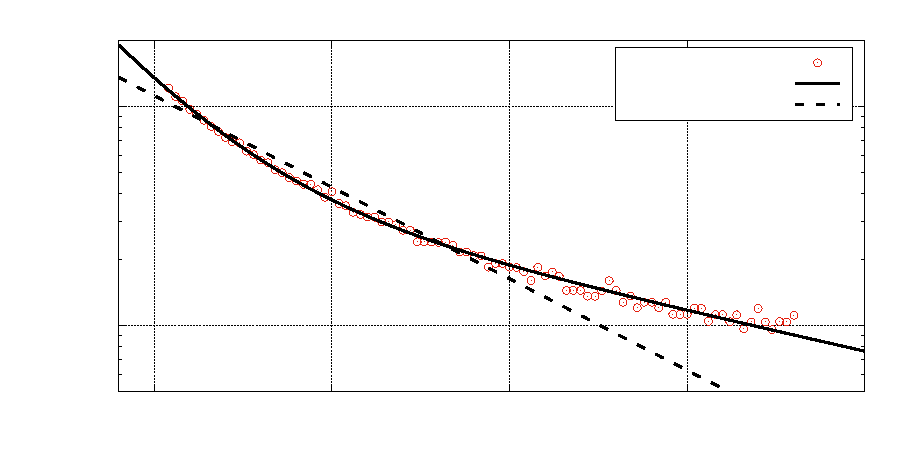
\includegraphics{peaks}}%
    \gplfronttext
  \end{picture}%
\endgroup
